\documentclass[../main/main.tex]{subfiles}

\newdate{date}{15}{10}{2020}


\begin{document}


\marginpar{ \textbf{Lecture 5.} \\  \displaydate{date}. \\ Compiled:  \today.}


\subsection{SIRS Model}
We now introduce another model, in which we take into account that during the years the \textbf{immune system may lose the ability to recognize a known pathogen}. This immunity could have been acquired via either a vaccine, or having recovered from that disease itself. Moreover, there could be the possibility that viruses mutate, as it occurs with the seasonal influenza, and so antibodies are not able to recognize it any more. Hence, let us build a model in which after an individual is recovered, can become again susceptible after a certain period of time.

The SIRS Model allows to interpolate between SIR (\( w=0 \)) and SIS (\( w \rightarrow \infty  \)), where $w$ is the \textbf{waning immunity rate}, namely the rate at which we lose our ability to defend ourselves from a certain pathogen. We can end up again into either an absorbing, with no more disease, or endemic state, where it keeps on circulating.
The transitions for this model are:
\begin{equation}
\begin{split}
 S + I &\overset{\beta }{\rightarrow } I + I   \\
 I & \overset{\mu }{\rightarrow } R  \\
 R & \overset{w}{\rightarrow } S
\end{split}
\end{equation}
In particular, the differential equations that describe the model are:
\begin{equation}
  \begin{split}
    \dv{s}{t} &= \alpha + w r - \beta  s i - \alpha s \\
  \dv{i}{t} &= \beta s i - \mu i - \alpha i \\
  \dv{r}{t} &= \mu i - w r - \alpha r
\end{split}
\end{equation}
In this case, the \textbf{endemic state} can be found by setting the derivatives equal to zero.

One may note that the transition \( R \rightarrow S \) does not affect the \( I \), so it holds that for the \textbf{infectious period}:
\begin{equation}
  \tau = \frac{1}{\alpha + \mu }
\end{equation}
while the $ \mathbf{R_0} $ factor is:
\begin{equation}
  R_0 = = \beta \tau = \frac{\beta }{\alpha + \mu }
\end{equation}
In addition, the equilibrium values \( s^* \), \( i^* \) and \( r^* \) can be easily obtained using the same arguments as of the SIR model with demography.

\subsection{SEIR Model}

In reality people do not become instantaneously infectious, but there is a \textbf{latent period} which is the time between infection and becoming infectious. Indeed, the pathogen replication takes time, i.e. viral load is too low to be able to transmit the infection. This argument leads us to introduce the \textbf{S}\textit{usceptible},  \textbf{E}\textit{xposed}, \textbf{I}\textit{nfected}, \textbf{R}\textit{ecovered} model, where the class \textbf{E} takes into account that a person has already contracted the disease, hence is not susceptible anymore, but is not able to spread it yet.

Moreover, this period can be extremely heterogeneous depending on the disease: it can take from few hours to years, such as the case for $HIV$ or, even longer, $TBC$. In the latter, latent periods might appear to be even longer than an individual's lifespan, with the result that he may have contracted the disease, but the death occurs for other causes before the onset of any symptom.

It is important to remind that the \textbf{latent period} is \textbf{not the same} of the \textbf{incubation period} (see Fig. \ref{fig:05_1}). An individual can be infectious before symptoms. For instance, there might be a \textbf{pre-syntomatic infection period} as it occurs in the case of COVID-19! This explains, once again, why medical status is different from the infection status.

\begin{figure}[h!]
\centering
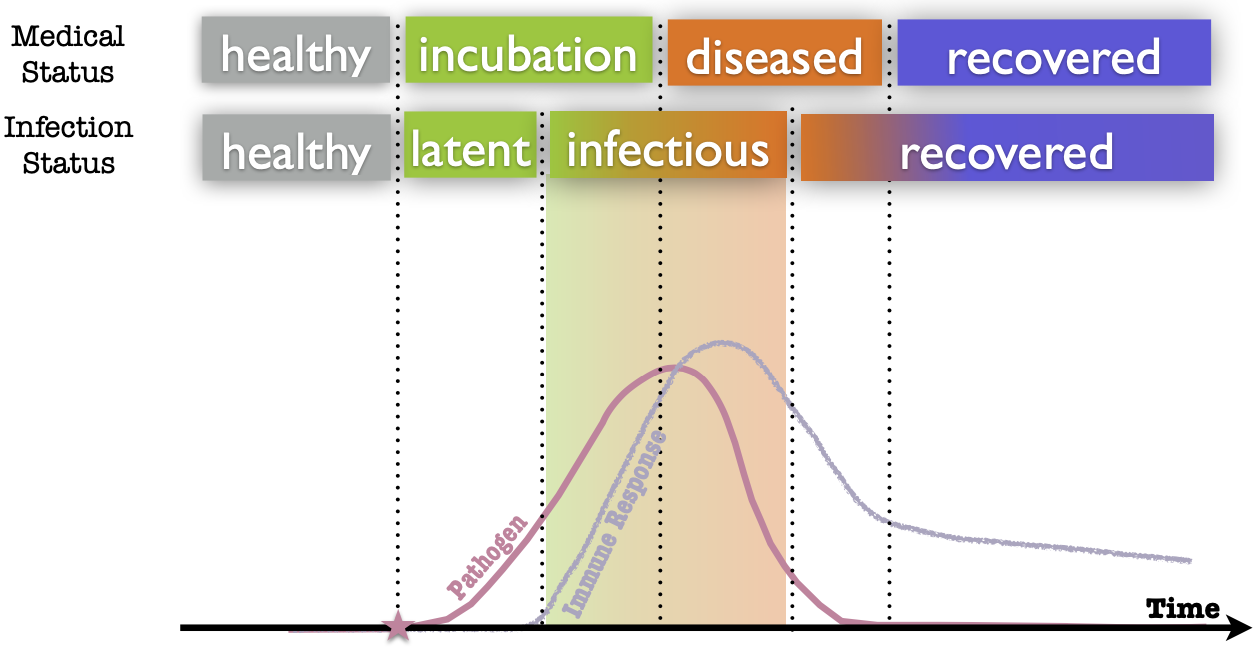
\includegraphics[width=0.7\textwidth]{../lessons/image/05/1.png}
\caption{\label{fig:05_1} Difference between infection status and medical status.}
\end{figure}

The transition for the \textbf{SEIR} model are:
\begin{equation}
\begin{split}
 S + I &\overset{\beta }{\rightarrow } I + E   \\
 E & \overset{\sigma }{\rightarrow } I  \\
 I & \overset{\mu }{\rightarrow } R
\end{split}
\end{equation}
with the equations:
\begin{equation}
  \begin{split}
    \dv{s}{t} &= \alpha -\beta s i - \alpha s \\
  \dv{e}{t} &= \beta s i - (\alpha + \sigma )e \\
  \dv{i}{t} &= \sigma e - (\alpha + \mu )i \\
  \dv{r}{t} &= \mu i - \alpha r
\end{split}
\end{equation}
Hence, the spreading is delayed due to the time spent in \( E \) class.

The \textbf{endemic state} is:
\begin{equation}
\begin{split}
s^*  &=  \frac{(\alpha +\mu )(\alpha + \sigma )}{\beta \sigma } = \frac{1}{R_0} \\
e^* &= \frac{\alpha (\alpha +\mu )}{\beta \sigma } (R_0 -1)\\
i^* &= \frac{\alpha }{\beta } (R_0 -1)
\end{split}
\end{equation}
For very short latent time (\( \sigma \rightarrow \infty  \)) we recover the endemic state of the SIR.

The \( \mathbf{R_0} \) factor is:
\begin{equation}
  R_0 = \frac{\beta \sigma }{(\alpha + \mu )(\alpha +\sigma )}
\end{equation}
Since latent time is way shorter than demography one, usually \( \frac{\sigma }{\sigma + \alpha } \simeq 1 \), hence \( R_0 = \frac{\beta }{\alpha + \mu } \) as in the SIR with demography.\\

One may object that, given that the infectious period and $R_0$ are similar between SEIR and SIR, adding the Exposed class may seem an unnecessary complication. However, if we look at the time evolution, at the \textbf{early stages} there is a huge difference between SEIR and SIR model:
\begin{equation}
\begin{split}
  i_{SEIR} (t) & \approx e^{\qty(\sqrt{4(R_0-1)\sigma \mu  + (\sigma + \mu )^2} -(\sigma +\mu ))t/2 } \approx i_0 e^{\qty(\sqrt{R_0} -1 ) \mu t} \\
    i_{SIR} (t) &\approx i_0 e^{(R_0-1) \mu t}
\end{split}
\end{equation}
Even if the behavior at the steady state is similar, the temporal evolution of the prevalence of SEIR model is actually slower than the one using SIR. This has surely to be taken into account in policy making, given its important implications.

The SEIR can be the starting point for modeling realistic diseases: i.e. Covid-19 (see Fig. \ref{fig:05_2}).
\begin{figure}[h!]
\centering
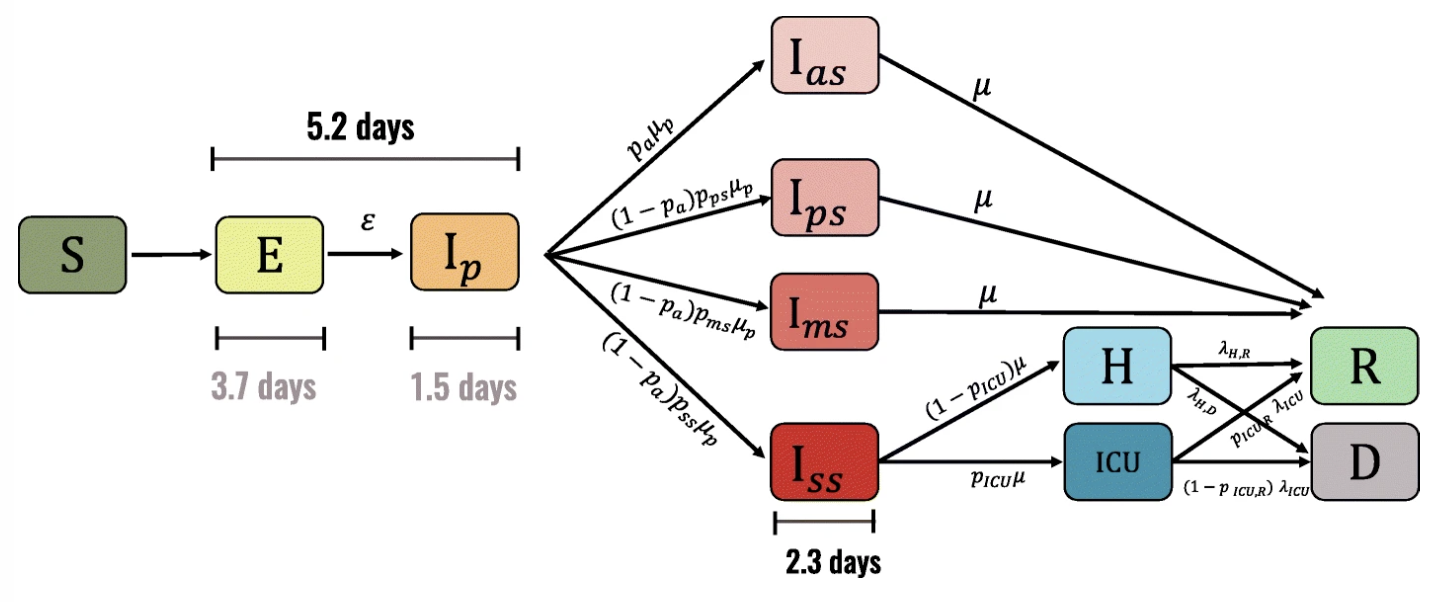
\includegraphics[width=0.7\textwidth]{../lessons/image/05/2.png}
\caption{\label{fig:05_2} Model for Covid-19.}
\end{figure}

\section{Summary of compartmental models in well-mixed populations}
Let us summarize all the compartmental models in well-mixed populations we have tackled so far:
\begin{itemize}
\item we solved the \textbf{SI model} analytically, and observed that the growth is the one of a sigmoid:
\begin{equation*}
  i(t) = \frac{i_0 e^{\beta t} }{1-i_0 + i_0 e^{\beta t} }
\end{equation*}
In the early stages we observe an exponential growth, governed by \( \beta  \), that always saturates at 1;

\item in the \textbf{SIS model} things starts to change. We have an \textbf{endemic} (meta-stable) \textbf{state}:
\begin{equation*}
  i(\infty) = \frac{\beta -\mu }{\beta }
\end{equation*}
which is a sort of \textbf{dynamical equilibrium} we reach. We can define an \textbf{epidemic threshold} $\beta_c$ according to which epidemics might spread or not:
\begin{equation*}
  \beta > \beta _c = \frac{\mu }{\expval{k} }
\end{equation*}
if $\beta> \beta_c$ then no exctinction for the epidemics occurs.

\item for the \textbf{SIR model} equations cannot be solved analytically. However, we observe \textbf{no endemic state} and the \textbf{epidemic threshold} is once again:
\begin{equation*}
  \beta > \beta _c = \frac{\mu }{\expval{k} }
\end{equation*}

\item then, in the \textbf{SIRS model} we introduced \textbf{waning immunity}. This model interpolates between SIR and SIS model. We do observe \textbf{endemic state} and the \textbf{infectious period} is:
\begin{equation*}
  \tau = \frac{1}{\alpha + \mu }
\end{equation*}
and moreover:
 \begin{equation*}
   R_0 = \frac{\beta }{\alpha + \mu }
 \end{equation*}

\item finally, we discussed \textbf{SEIR model} in which we included a \textbf{latent period}. We have that:
\begin{equation*}
  R_0 = \frac{\beta \sigma }{(\alpha + \mu )(\alpha +\sigma )}
\end{equation*}
and the Exposed class has the effect to slow down the spreading.
\end{itemize}











\chapter{Network Science - Basics}

\section{Main definitions}

When we talk about Network Science, as the name would suggest, we study \textbf{Networks} that, in math, are also known as graph.
A \textbf{Graph} $G(V,E)$ is simply an object that is composed by a set of \textbf{nodes} (vertices) \( V \) and a set of \textbf{links} (edges) \( E \):
\begin{itemize}
\item \textbf{nodes} represent the \emph{entities} \( V=[\dots,i,j,k,\dots] \) involved in some relationship. These might be entries, people belonging to a social network and so forth. The \textbf{number of nodes} is \( N= \abs{V}  \);

\item \textbf{links} represent the relationships between entities \( E=[\dots,(i,j),(i,k),\dots] \). The \textbf{number of links} is \( L= \abs{E}  \).
\end{itemize}

Links can be of different kinds and so networks: the basic distinction is between \textbf{undirected} and \textbf{directed} links. The former ones can be thought as directed edges, but with arrows pointing in both directions, i.e. to both node of the pair. While the second ones do have a direction according to which sense the relationship represented by the link holds.\\
Another important distinction is between \textbf{unweighted} and \textbf{weighted} links. The latter ones can be exploited to take into account the possibility that some nodes can be more connected than the others, therefore \textbf{weights} follow. In a certain sense, it describes the "strength" of the link between two nodes.\\

Another important quantity is the \textbf{network density} (connectance), that is the fraction of links present normalized to all the possible pairs, and for undirected networks is:
\begin{equation}
  d = \frac{2L}{N(N-1)}
\end{equation}
\textbf{Real networks} usually have a very low density, so are \textbf{sparse systems} (\( L \ll N^2 \)).

A graph, mathematically, can be represented by the mean of a matrix. It is the so called \textbf{adjacency matrix} \( A \) of the network, where:
\begin{itemize}
\item \( a_{ij} = 1 \), if a link between nodes \( i \) and \( j \) exists;
\item \( a_{ij} = 0 \) otherwise.
\end{itemize}
Many mathematical tools can be used to determine the properties of the system alongside with this matrix, as an example we may want to compute its spectrum in order to obtain the largest eigenvalue. Moreover, one should note that the matrix is symmetrical for undirected and unweighted graphs, i.e. \( a_{ij} = a_{ji} \).
However, as we already told, real networks are usually sparse, therefore the adjacency matrix will be filled for large part by zeros. Hence in order to store graphs in a computer efficiently, it is better to use other tools such as adjacency lists, etc.

Two nodes that share a link are defined "connected", "adjacent", "neighbors". In particular, the \textbf{neighborhood} of node \( i \) is the set of nodes connected to \( i \).
The number of neighbors \( k_i \) of each node \( i \) is what is called the \textbf{degree} of the node $i$. This is the basic measure that we are going to encounter so many times. Once we have defined the degree, the next step is to define what is the \textbf{average degree} over the entire network (undirected case):
\begin{equation}
  \expval{k} = \frac{1}{N} \sum_{i=1}^{N} k_i, \qquad \text{or} \qquad \expval{k} = \frac{2L}{N} = d(N-1)
\end{equation}

The next definition is the one of \textbf{path}, which is a sequence of links which permits to go from node \( i \) to node \( j \) following edges. Another relevant quantity is the so called \textbf{shortest path} between \( i \) and \( j \), it is important since it gives us the idea of how big the network is. In particular, the \textbf{distance} \( l_{ij} \) represents the length of the shortest path between \( i \) and \( j \). There could be multiple shortest paths between \( i \) and \( j \).
The shortest path of maximum length in the network is defined as \textbf{diameter}:
\begin{equation*}
  l_{max} = \max_{ij} l_{ij}
\end{equation*}
Another measure we may want to introduce is the \textbf{average} (shortest) \textbf{path length}:
\begin{equation*}
  \expval{I} = \frac{\sum_{ij}^{} l_{ij} }{N(N-1)}
\end{equation*}

The network is said to be \textbf{connected} if every possible couple of nodes is reachable through a path. Otherwise, each connected part is defined as a \textbf{connected component}.



Now, let us see some examples of networks, such as “The Oracle of Bacon”, or the so called “Erdos Number”. The first one is a site that, given the name of an actor, returns the distance between this actor and Kevin Bacon,  in unit of costarring movies. This quantity is indeed computed by taking into account the network of actors, linked by common movies in which they starred. The \textbf{Erdos Number} instead is the "academical version" for the "Oracle of Bacon": we compute the distance, in terms of collaborations in publications, between a given researcher and the mathematician Paul Erdos through the publications network. The most surprising fact is that, for both examples, the distance is very low! Therefore a question arises: why such short distances in such large networks?
In particular, real networks are smaller (i.e. shorter) than one would expect. This is pointed out by the idea of the “Six degrees of separation”. It refers to an experiment that was run in the '60s by Stanley Milgram: he gave a postcard to a person on the West Coast, with the instructions that it had to be delivered to a place situated in the East Coast. The main goal was to count how many people would receive that postcard, given the rule that it was allowed to give the postcard to acquaintances of the actual possessor. It was discovered that this postcard actually was delivered to 6 people before reaching the destination.
This is what is called the \textbf{small world phenomena}. When we study the average path length, for some networks we may find that $\expval{I} \sim ln(N)$ or, in some cases even $\expval{I} \sim ln(ln(N))$. This is extremely important in the spreading of diseases, since we are able to cover the whole system in few steps.

\end{document}
